\documentclass{article}

\usepackage[utf8]{inputenc}
\usepackage[T1]{fontenc}
\usepackage{hyperref}
\usepackage{tabularx}
\usepackage{array}
\usepackage{fancyhdr}
\usepackage{graphicx}
\usepackage[a4paper]{geometry}
\usepackage{multicol}
\usepackage{listings}
\usepackage{tabto}

\title{Projet de BigData \\ Les bases NoSQL}
\author{par Jordan Baudin, Corentin LeGuen et Geoffrey Spaur}
\date{11 janvier 2018}
\pagestyle{fancy}
\lhead{Projet de BigData - Les bases NoSQL \\ \textbf{M2GIL} - Jordan Baudin, Corentin LeGuen et Geoffrey Spaur}
\rhead{
\includegraphics[scale=0.5]{logo_univ_rouen.png}}
\setlength{\headsep}{1cm}
\begin{document}

\maketitle
\newpage
\tableofcontents{}
\newpage
\section{Présentation}
  \paragraph{}
  Ce projet a pour but de comparer différentes bases de données NoSQL.
  Nous allons prendre les bases données CouchBase et MongoDB.
  
 \newpage
\section{La base de donnée CouchBase}
\subsection{Les modalités d’installation}
  \paragraph{} TODO
\subsection{Les méthodes d’insertion de données}
  \paragraph{} TODO
\subsection{Le langage de recherche}
  \paragraph{} TODO
\subsection{L’indexation interne}
  \paragraph{} TODO
\subsection{Le support de la concurrence d’accès}
  \paragraph{} TODO
\subsection{L’architecture du système}
  \paragraph{} TODO
\subsection{Les techniques de distribution}
  \paragraph{} TODO
  
  
  
\newpage
\section{La base de donnée MongoDB}
\subsection{Les modalités d’installation}
  \paragraph{Téléchargement} Pour l'installation de MongoDB, il vous suffira
  dans un premier temps de \href{https://www.mongodb.com/download-center#community}{télécharger} 
  l'archive contenant MongoDB.
  \paragraph{} Après le téléchargement de l'archive, vous pourrez la décompresser. Avant
  de lancer le serveur, il vous faudra créer le dossier \textbf{/data/db}. Ce dossier
  contiendra toutes les bases de MongoDB.
  \paragraph{} Enfin vous pouvez lancer le serveur MongoDB avec la commande:
  \begin{lstlisting}
  $ ./bin/mongod
  \end{lstlisting}
  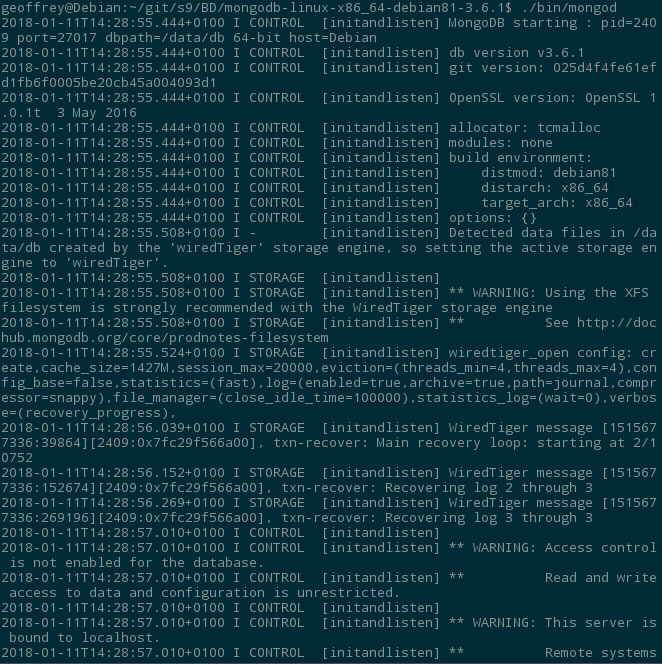
\includegraphics[scale=0.8]{mongodb/lancement_mongo.png}\\
  Vous pourrez ensuite accéder à MongoDB en lançant le client grâce à la commande suivante:
  \begin{lstlisting}
  $ ./bin/mongo
  \end{lstlisting}
  
  
\subsection{Les méthodes d’insertion de données}
  \paragraph{Création de la base} Avant toute insertion, lancez le client MongoDB
  avec la commande précédente. Nous allons ajouter une nouvelle base de donnée. 
  Vous pouvez lister les différentes base de données déjà présentes avec la commande:
  \begin{lstlisting}
  > show dbs
  \end{lstlisting}
  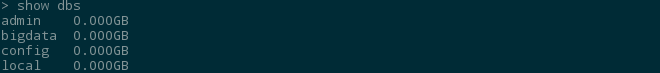
\includegraphics[scale=0.8]{mongodb/show_dbs.png}\\
  Puis pour créer et/ou utiliser notre base de donnée, utilisez:
  \begin{lstlisting}
  > use DATABASE
  \end{lstlisting}
  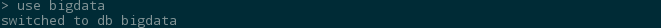
\includegraphics[scale=0.8]{mongodb/use_dbname.png}\\
  Vous pouvez lister vos collections de document avec la commande suivante:
  \begin{lstlisting}
  > show collections
  \end{lstlisting}
  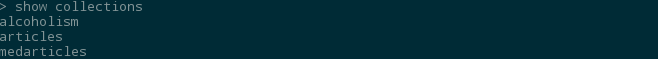
\includegraphics[scale=0.8]{mongodb/show_collections.png}\\
  
  \paragraph{Insertion de documents}
  Vous pouvez maintenant sortir du client MongoDB. Vos documents doivent être en
  format json sous forme d'objet. Vous trouverez un exemple avec le fichier 
  \emph{prettyAlcoholism.json}. Nous allons utiliser la commande
  \emph{mongoimport} afin d'ajouter nos document dans notre base:
  \begin{lstlisting}
  $ ./bin/mongoimport --db bigdata --collection medarticles 
  --file ../Projet/prettyAlcoholism.json
  \end{lstlisting}
  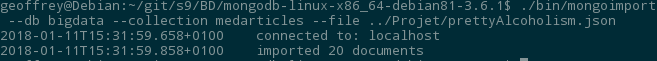
\includegraphics[scale=0.8]{mongodb/insertiondedoc2.png}\\
  \paragraph{} Vous pouvez cependant ajouter des document directement à partir
  du client MongoDB avec les commandes \emph{import} ou \emph{importMany}.
  Ces commandes sont utiles dans le cas où nous avons peu de document ou des
  document de petites tailles.
  
\subsection{Le langage de recherche}
  \paragraph{} Pour rechercher des documents dans MongoDB, nous utiliserons la 
  fonction \emph{find()} sur nos collections. Cette commande peut prendre jusqu'à
  deux arguments sous format JSON:
  \begin{itemize}
    \item Le premier permet de déterminer la clause \textbf{where}.
    \item La seconde permet de spécifier les champs à afficher.
  \end{itemize}
  \subsubsection{Les conditions}
    \paragraph{} Vous pouvez effectuer une recherche en indiquant la valeur d'un
    champs comme ceci:\\
    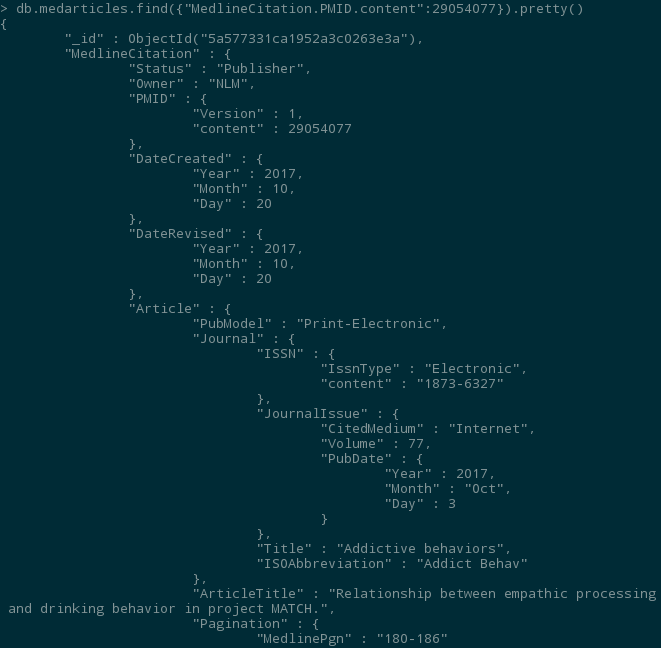
\includegraphics[scale=0.8]{mongodb/recherche_find1.png}\\
    En ajoutant la fonction \emph{pretty()}, le résultat sera indenté.
    Vous pouvez utiliser les tableaux \emph{\$and} et \emph{\$or} afin de constituer
    des recherches plus complexes.
  \subsubsection{L'affichage}
    \paragraph{} Vous pouvez aussi n'afficher que certain champs dans le résultat
    de votre recherche:\\
    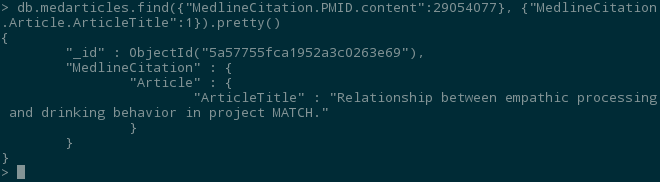
\includegraphics[scale=0.8]{mongodb/recherche_find2.png}\\
  
\subsection{L’indexation interne}
  \paragraph{} Pour chaque document ajouter dans une collection, MongoDB lui ajoute
  un champs \emph{\_id}. C'est ce champs qui sera indexé par défaut. Il est 
  possible de lister tous les indexes d'une collection avec la commande suivant:
  \begin{lstlisting}
  > db.medarticles.getIndexes()
  \end{lstlisting}
  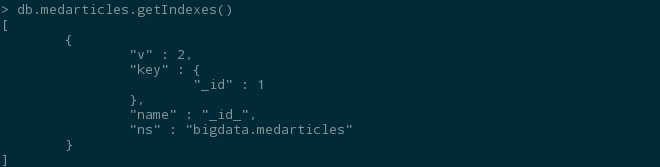
\includegraphics[scale=0.8]{mongodb/getindexes.png}\\
  
  \paragraph{} Vous pouvez cependant ajouter vos propres indexes avec la commande
  \emph{ensureIndex()}. L'objet JSON passé en argument doit être une liste de \textbf{int}.
  Le nom doit être le champs à indexer et le \textbf{int} doit être égal à 1 ou -1; 
  la valeur 1 correspond à un tri ascendant et la valeur -1 à un tri descendant.
  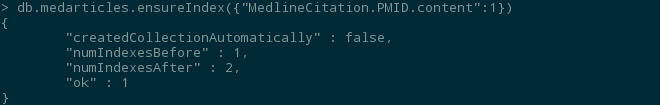
\includegraphics[scale=0.8]{mongodb/ensureIndex.png}\\
  
  \paragraph{} Afin de mesurer l'impact de vos indexes, à chaque recherche vous pouvez
  ajouter la méthode \emph{explain}:\\
  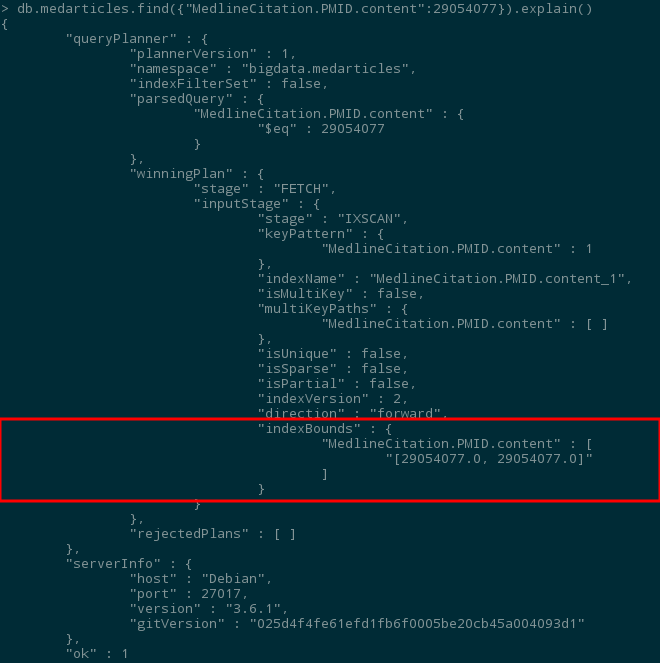
\includegraphics[scale=0.8]{mongodb/find_explain2.png}\\
\subsection{Le support de la concurrence d’accès}
  \paragraph{} MongoDB support totalement la concurrence d'accès.
  Il permet à plusieurs clients de lire et écrire les mêmes données.
  MongoDB gère la concurrence à l'aide de verrous. Certaines opérations entraînent
  un verrouillage de la collection ou même de la base de données. Par exemple
  les opérations d'insertion, de suppression, de modification ou encore de
  création d'index entraînent un verrouillage de la base de données.
\subsection{L’architecture du système}
  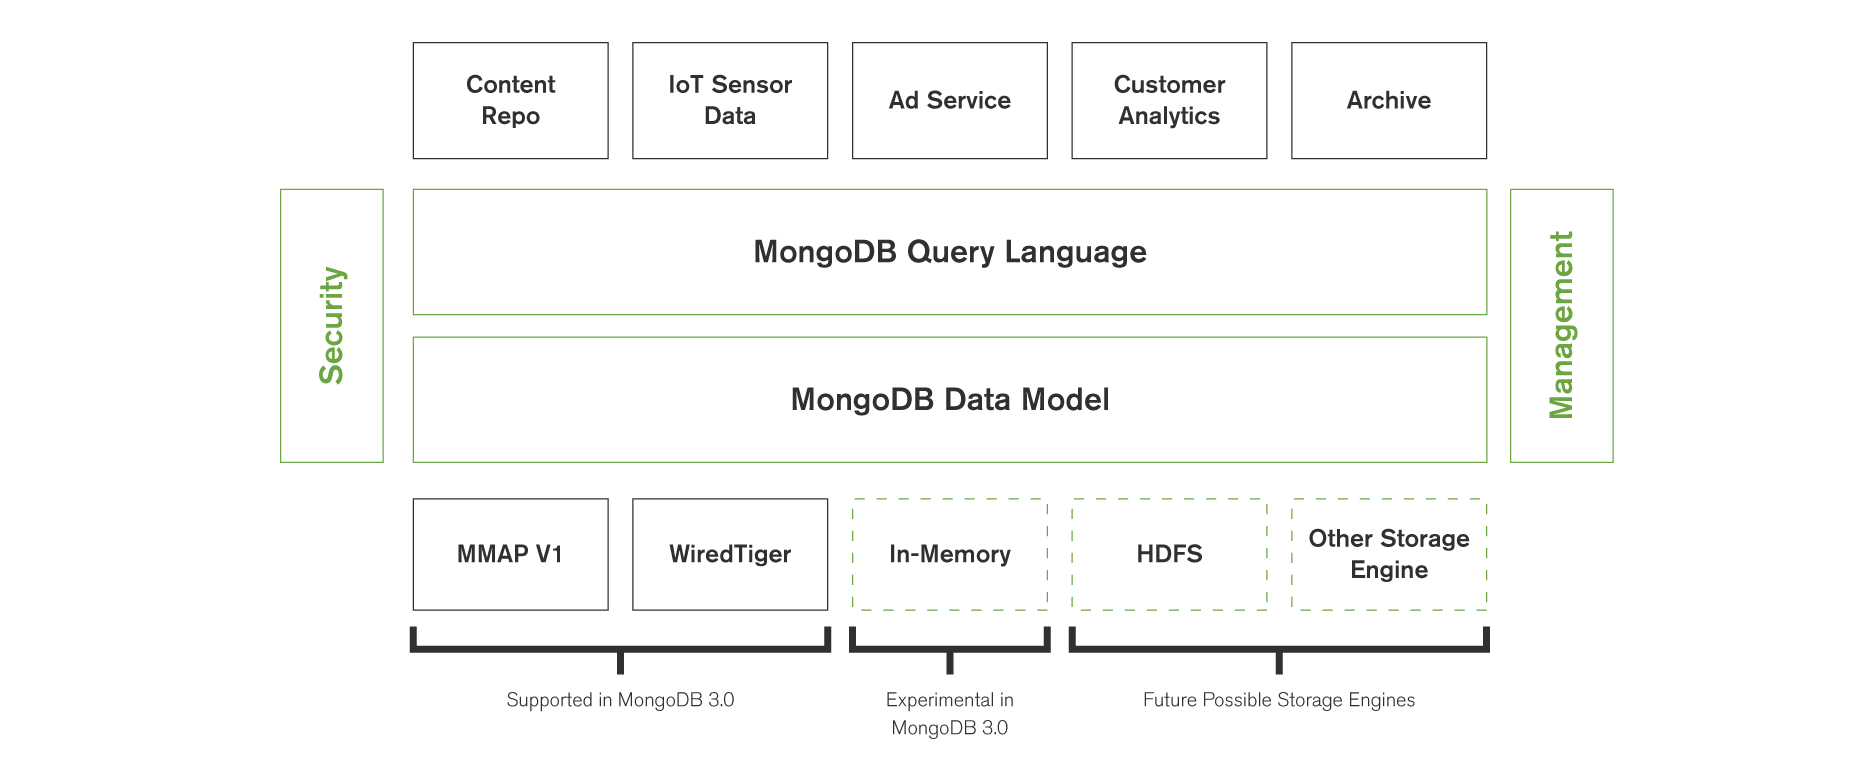
\includegraphics[scale=0.215]{mongodb/mongodb-arch-diag.png}\\
\subsection{Les techniques de distribution}
  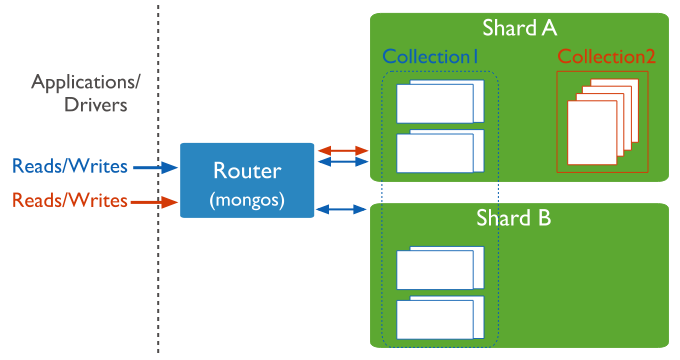
\includegraphics[scale=0.7]{mongodb/sharded-mongodb.png}\\

\newpage
\section{Conclusion}
  \paragraph{} TODO
  
\end{document}